\documentclass[tikz,border=12pt]{standalone}
\usepackage[T1]{fontenc}
\usepackage{lmodern}
\usepackage{tikz}
\usetikzlibrary{arrows.meta, positioning, calc, fit}

\definecolor{TitleBar}{RGB}{220,220,220}
\definecolor{GrayBorder}{RGB}{145,145,145}
\definecolor{GrayFill}{RGB}{246,246,246}
\definecolor{BlueFill}{RGB}{210,225,245}
\definecolor{BlueBorder}{RGB}{70,105,175}
\definecolor{OrangeFill}{RGB}{255,235,205}
\definecolor{OrangeBorder}{RGB}{205,125,35}
\definecolor{GreenFill}{RGB}{210,238,210}
\definecolor{GreenBorder}{RGB}{75,150,80}
\definecolor{RedFill}{RGB}{248,215,215}
\definecolor{RedBorder}{RGB}{180,70,70}
\definecolor{PurpleFill}{RGB}{232,220,248}
\definecolor{PurpleBorder}{RGB}{125,90,170}
\definecolor{MutedText}{RGB}{90,90,90}

\tikzset{
  every node/.style={font=\sffamily},
  arr/.style={-{Stealth[length=6pt,width=5pt]}, line width=1.0pt, black},
  note/.style={font=\sffamily\footnotesize, align=center, text=MutedText},
  pc/.style={draw=BlueBorder, fill=BlueFill, rounded corners=4pt,
             minimum width=92pt, minimum height=34pt, align=center},
  pathA/.style={draw=OrangeBorder, fill=OrangeFill, rounded corners=4pt,
                minimum width=106pt, minimum height=34pt, align=center},
  pathB/.style={draw=GreenBorder, fill=GreenFill, rounded corners=4pt,
                minimum width=106pt, minimum height=34pt, align=center},
  ret/.style={draw=PurpleBorder, fill=PurpleFill, rounded corners=4pt,
              minimum width=92pt, minimum height=34pt, align=center},
  stackbox/.style={draw=GrayBorder, fill=GrayFill, rounded corners=5pt,
                   minimum width=165pt, minimum height=52pt, align=center},
  stackentry/.style={draw=RedBorder, fill=RedFill, rounded corners=3pt,
                     minimum width=120pt, minimum height=20pt, align=center,
                     font=\sffamily\footnotesize},
  activeentry/.style={draw=GreenBorder, fill=GreenFill, rounded corners=3pt,
                      minimum width=120pt, minimum height=20pt, align=center,
                      font=\sffamily\footnotesize},
  lane/.style={draw=GrayBorder, fill=white, rounded corners=2pt,
               minimum width=24pt, minimum height=18pt,
               font=\sffamily\scriptsize},
  laneon/.style={lane, draw=GreenBorder, fill=GreenFill},
  laneoff/.style={lane, draw=GrayBorder, fill=white, text=MutedText}
}

\newcommand{\masklanes}[5]{%
  \node[#1] (#5a) at (0,0) {T3};
  \node[#2, right=2pt of #5a] (#5b) {T2};
  \node[#3, right=2pt of #5b] (#5c) {T1};
  \node[#4, right=2pt of #5c] (#5d) {T0};
}

\begin{document}
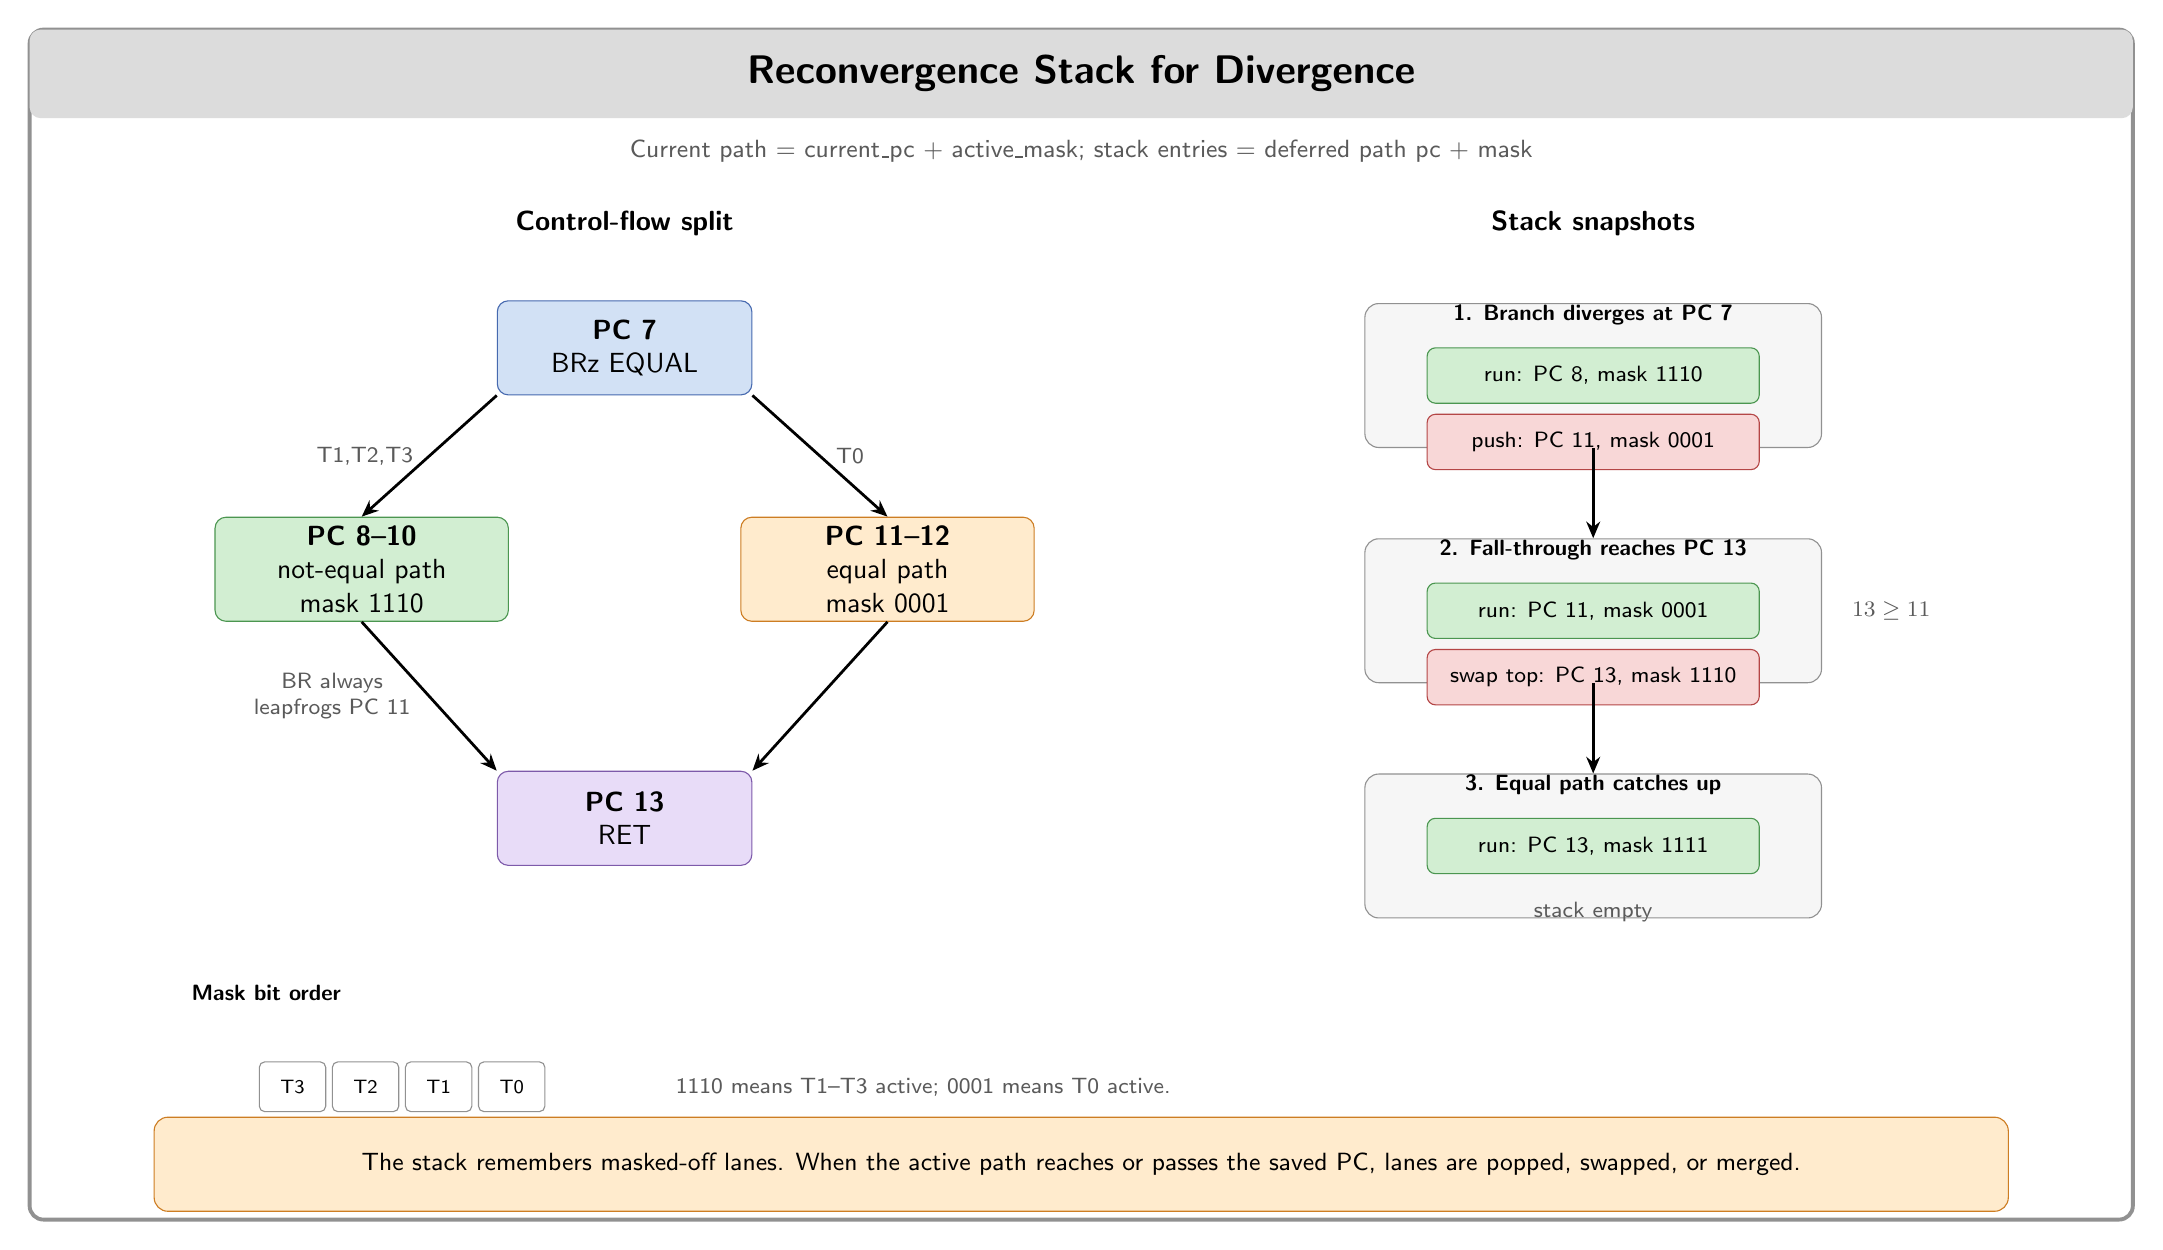
\begin{tikzpicture}[x=1pt,y=1pt]

% Outer slide frame
\draw[line width=1.4pt, GrayBorder, fill=white, rounded corners=5pt]
  (0,0) rectangle (760,430);
\fill[TitleBar, rounded corners=4pt] (0,398) rectangle (760,430);
\node[font=\sffamily\Large\bfseries] at (380,414)
  {Reconvergence Stack for Divergence};
\node[font=\sffamily\small, text=MutedText] at (380,386)
  {Current path = current\_pc + active\_mask; stack entries = deferred path pc + mask};

% Column headings
\node[font=\sffamily\bfseries] at (215,360) {Control-flow split};
\node[font=\sffamily\bfseries] at (565,360) {Stack snapshots};

% Control-flow graph
\node[pc] (br) at (215,315) {\textbf{PC 7}\\BRz EQUAL};
\node[pathB] (fall) at (120,235) {\textbf{PC 8--10}\\not-equal path\\mask 1110};
\node[pathA] (equal) at (310,235) {\textbf{PC 11--12}\\equal path\\mask 0001};
\node[ret] (join) at (215,145) {\textbf{PC 13}\\RET};

\draw[arr] (br.south west) -- node[note, left=2pt] {T1,T2,T3} (fall.north);
\draw[arr] (br.south east) -- node[note, right=2pt] {T0} (equal.north);
\draw[arr] (fall.south) -- node[note, left=3pt] {BR always\\leapfrogs PC 11} (join.north west);
\draw[arr] (equal.south) -- (join.north east);

% Lane legend
\node[font=\sffamily\footnotesize\bfseries, anchor=west] at (55,82) {Mask bit order};
\begin{scope}[shift={(95,48)}]
  \masklanes{lane}{lane}{lane}{lane}{legend}
\end{scope}
\node[note, anchor=west] at (230,48) {1110 means T1--T3 active; 0001 means T0 active.};

% Stack snapshot 1
\node[stackbox] (s1) at (565,305) {};
\node[font=\sffamily\bfseries\footnotesize] at (565,327) {1. Branch diverges at PC 7};
\node[activeentry] at (565,305) {run: PC 8, mask 1110};
\node[stackentry] at (565,281) {push: PC 11, mask 0001};

% Stack snapshot 2
\node[stackbox] (s2) at (565,220) {};
\node[font=\sffamily\bfseries\footnotesize] at (565,242) {2. Fall-through reaches PC 13};
\node[activeentry] at (565,220) {run: PC 11, mask 0001};
\node[stackentry] at (565,196) {swap top: PC 13, mask 1110};
\node[note, anchor=west] at (655,220) {$13 \ge 11$};

% Stack snapshot 3
\node[stackbox] (s3) at (565,135) {};
\node[font=\sffamily\bfseries\footnotesize] at (565,157) {3. Equal path catches up};
\node[activeentry] at (565,135) {run: PC 13, mask 1111};
\node[font=\sffamily\footnotesize, text=MutedText] at (565,111) {stack empty};

\draw[arr] (s1.south) -- (s2.north);
\draw[arr] (s2.south) -- (s3.north);

% Key takeaway
\node[draw=OrangeBorder, fill=OrangeFill, rounded corners=5pt,
      minimum width=670pt, minimum height=34pt, align=center,
      font=\sffamily\small] at (380,20)
  {The stack remembers masked-off lanes. When the active path reaches or passes the saved PC, lanes are popped, swapped, or merged.};

\end{tikzpicture}
\end{document}
